% Provenance (never printed): see sources/outline_sources.md (Year 1: gravity and its
% measurement, normal gravity; isostasy, Airy and Pratt; free-air and Bouguer anomalies;
% the geoid). Curves from figdata/bachelor-1/hypsometry.py and gravity_profiles.py;
% exercise and problem values in the Book 3 scratch calculator calc/ch11.py.
\chapter{地壳均衡与重力异常}\label{ch:b1:isostasy-gravity}

1840 年代，测量员在印度北部测量子午线弧时，遇到了一个
无法归咎于仪器的偏差。两个相距约 370 英里的测站之间，
一个是靠近喜马拉雅山脚的卡利亚纳，另一个是南方远处的卡利安普尔，
三角测量得出的\omterm{def:b1:spherical-astronomy:geographic}{纬度}差，超出了
由天文观测得出的\omterm{def:b1:spherical-astronomy:geographic}{纬度}差 5.236 角秒。最明显的原因是
山脉：它们的引力使铅垂线偏向北方，天文学家正是依据铅垂线校准仪器。
1855 年，约翰·亨利·普拉特
计算了喜马拉雅山及其北侧高原的引力，
发现这一引力应使偏差达 15.885 角秒，
是观测值的三倍多。山脉的拉力远小于按其可见质量所应有的数值，
同年，乔治·艾里回答说，\omterm{def:b1:layered-earth:layers}{地壳}漂浮于较致密的层之上，
如同水上的一排木筏，使高地之下具有很深的
轻质岩石“根”。之后普拉特又提出另一种解释，认为
岩石因山下膨胀而变轻。两种解释至今仍被讲授：
山脉之下为轻质岩石，可补偿其质量。本章把这一想法
转化为数值计算，
并说明如何借助精确到其数值百万分之一的重力测量，
揭示地形起伏之下隐藏的质量。
% ledger: pratt:himalaya, airy:1855, pratt:1871

\begin{recall}
牛顿万有引力定律给出球外的场 $g = GM/r^2$，
其中 $M$ 为球体质量；场由引力势导出，而等势面
处处与场垂直（物理课程）。静止流体中，
压强随深度增加，满足 $\mathrm dp/\mathrm dz = \rho g$，而
漂浮物体排开与自身重量相等的流体（物理学，本科一年级）。
\omterm{def:b1:layered-earth:lithosphere}{岩石圈}之下的\omterm{def:b1:layered-earth:lithosphere}{软流圈}在长时间尺度上会流动；\omterm{def:b1:layered-earth:layers}{地壳}
比其下方的\omterm{def:b1:layered-earth:layers}{地幔}轻（见\cref{ch:b1:layered-earth}；第 2 册，十一年级）。
\end{recall}

\section{重力及其测量}

地表重力加速度接近
\qty{9.8}{m.s^{-2}}，地质学家关心的变化
则小一百万倍。它们以旧的厘米–克–秒制中的一个单位计量，
即伽：$\qty{1}{Gal} = \qty{1}{cm.s^{-2}} = \qty{0.01}{m.s^{-2}}$，
故有
\[
  \qty{1}{\milli\gal} = \qty{e-5}{m.s^{-2}} \approx \num{e-6}\,g .
\]
% ledger: nist:gal
野外仪器能分辨千分之几毫伽。本章所研究的异常
幅度从埋藏矿体上方的不足一毫伽
到山脉上方的数百毫伽不等。

即使地球没有任何地形起伏，重力也不会处处相同。
地球自转，因此铅垂线或重力仪所感受到的，是
引力与自转离心效应之和；而且
地球是扁的，两极比赤道更靠近球心。
两种效应都使赤道处的重力比两极处弱。地质学家
将每个测量值都与一个包含上述效应的光滑参考值相比较。

\begin{definition}[正常重力]\label{def:b1:isostasy-gravity:normal-gravity}
\emph{正常重力}\index{正常重力}（$\gamma$）是一个模型地球的重力：
即具有地球质量与自转的旋转椭球体，其取法使
它的表面是其自身重力（引力与离心效应）的等势面。
该面上，正常重力仅依赖于\omterm{def:b1:spherical-astronomy:geographic}{纬度}。
\end{definition}

旋转椭球本身、其扁率，以及其参数如何拟合真实地球，
将在第 5 册中研究。这里只需要它的重力。

\begin{proposition}[正常重力公式]\label{prop:b1:isostasy-gravity:normal-formula}
在 1980 年采用的参考椭球上，
地理\omterm{def:b1:spherical-astronomy:geographic}{纬度} $\varphi$ 处的\omterm{def:b1:isostasy-gravity:normal-gravity}{正常重力}，其常用级数形式为
\[
  \gamma(\varphi) = \qty{9.780327}{m.s^{-2}}\,\bigl(1 + 0.0053024\sin^2\varphi
  - 0.0000058\sin^2 2\varphi\bigr).
\]
\end{proposition}
\admitted
% ledger: moritz:grs80

在赤道为 \qty{9.780327}{m.s^{-2}}，在
\ang{45} 处为 \qty{9.806200}{m.s^{-2}}，两极为 \qty{9.832186}{m.s^{-2}}，两者相差
\qty{5186}{\milli\gal}（自赤道至两极）。自转本身便解释了
其中大部分。取恒星日为 \qty{23.9345}{h}，角速度为
$\omega = 2\pi/\qty{86164}{s} = \qty{7.292e-5}{rad.s^{-1}}$，而赤道处的离心
加速度为 $\omega^2 a$，其中 $a = \qty{6378.137}{km}$，
即 \qty{0.0339}{m.s^{-2}}，合 \qty{3392}{\milli\gal}；其余
部分由扁率提供（见\cref{exo:b1:isostasy-gravity:2}）。
% ledger: earth:Trot, earth:Req, earth:geq, earth:gpole

重力测量有两种方式。\emph{绝对}重力仪使一个试验质量在真空室中下落，
并用激光干涉仪跟踪其自由落体，
以原子钟计时：加速度直接由距离与
时间得出。\emph{相对}重力仪是挂在弹簧上的质量块，其伸长
随重力而变；它轻便快速，但只能给出两地之间的
差值，而且会漂移，因此测量须返回一个
基站，其重力已知。最好的绝对仪器精度约为一
微伽，即 $g$ 的十亿分之一。
% ledger: ngs:absolute-gravity

\begin{inthefield}[陆地重力测量]
\begin{minipage}[t]{0.55\linewidth}\vspace{0pt}
重力测量是在各测站之间缓慢行进的过程。在每个测站，
地球物理学家将相对重力仪架设在三脚架上并调平，等待
弹簧稳定后读取数次；旁边的卫星定位
接收机记录测站的位置与高程。每隔几小时
测量队便返回基站，以便测出并扣除弹簧的漂移，
高程与重力同等重要：如下一节所示，
重力每升高一米减小 \qty{0.3086}{\milli\gal}，
因此高程误差 \qty{1}{cm} 会使读数偏差
\qty{3}{\micro\gal}。 % ledger: usgs73:reduction
\end{minipage}\hfill
\begin{minipage}[t]{0.42\linewidth}\vspace{0pt}
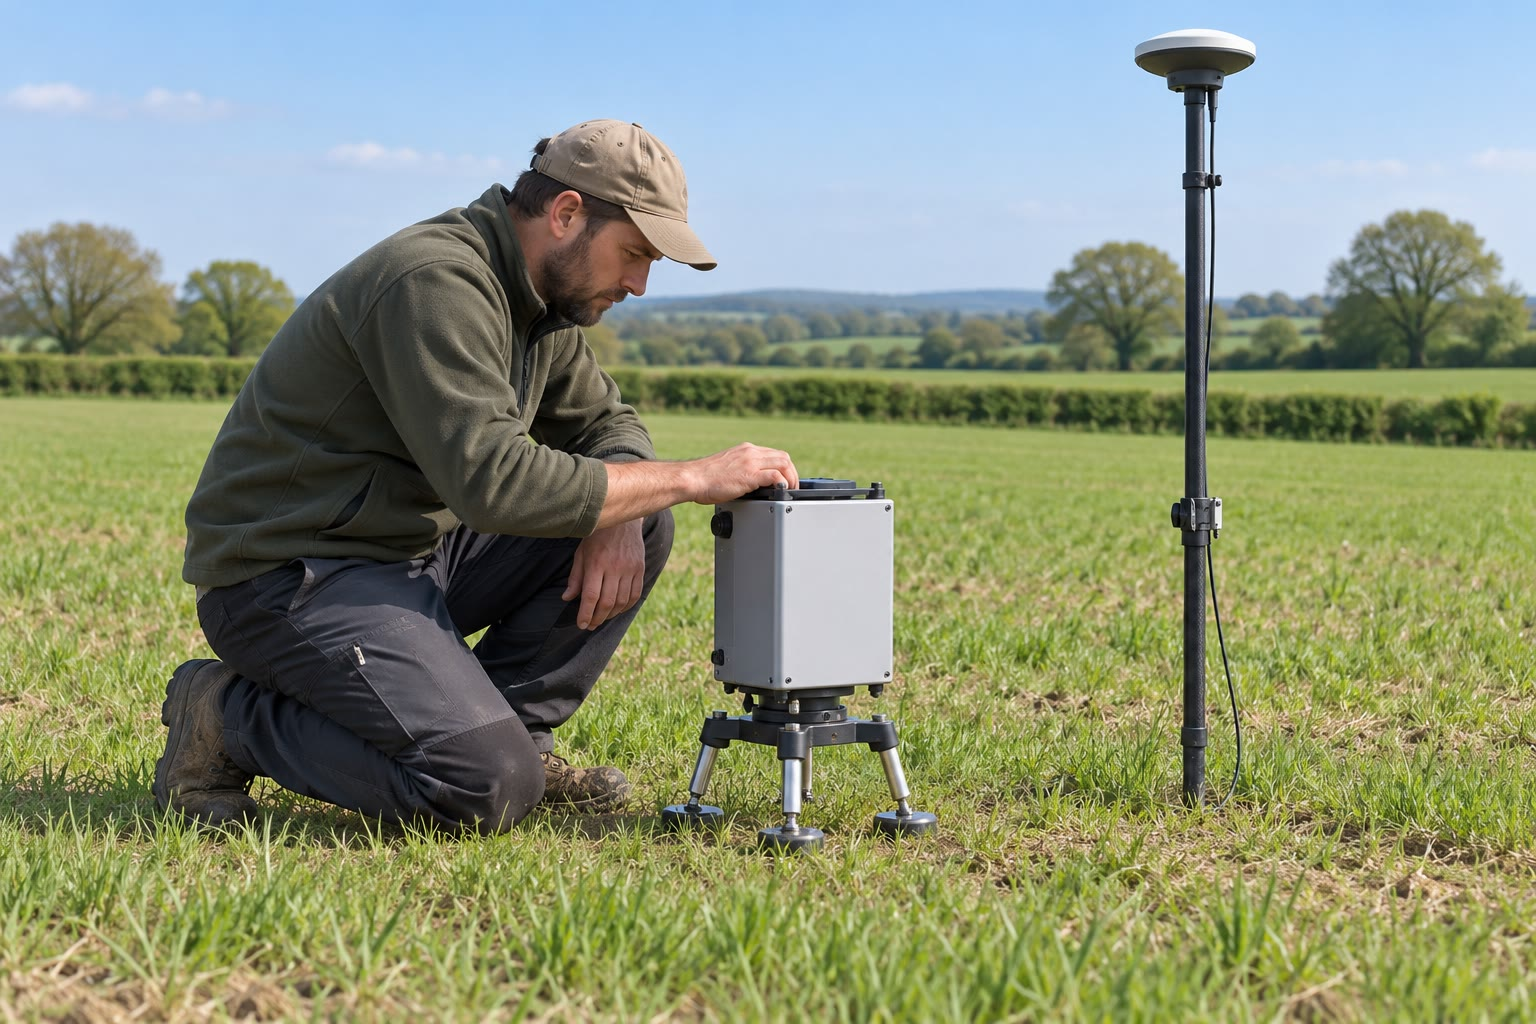
\includegraphics[width=\linewidth]{images/book3/ai/b1-gravity-survey.jpg}

{\scriptsize 三脚架上的相对重力仪，旁边是卫星定位
天线（AI 生成插图）。}
\end{minipage}
\end{inthefield}

\section{地壳均衡}

艾里和普拉特为喜马拉雅山所设想的补偿，
是地球外层一般状态的一个实例。

\begin{definition}[地壳均衡；补偿深度]\label{def:b1:isostasy-gravity:isostasy}
某区域处于\emph{地壳均衡}\index{地壳均衡}状态（或称\omterm{def:b1:layered-earth:layers}{地壳}均衡平衡），是指
存在一个深度，即\emph{补偿深度}\index{补偿深度}，
在该深度处，水平面上各点的压强均相同，
而与其上的地形起伏无关。补偿深度以下，岩石表现为
静止的流体；补偿深度以上，\omterm{def:b1:layered-earth:layers}{地壳}与\omterm{def:b1:layered-earth:layers}{地幔}的柱体则漂浮于其上。
\end{definition}

\begin{proposition}[补偿深度以上的质量相等]\label{prop:b1:isostasy-gravity:equal-mass}
若沿各柱体的重力 $g$ 相同，则某区域处于\omterm{def:b1:isostasy-gravity:isostasy}{地壳均衡}状态，
其\omterm{def:b1:isostasy-gravity:isostasy}{补偿深度}为 $z_c$，当且仅当每个单位
截面的竖直柱体，从地表向下直至 $z_c$，所含质量均相同。
\end{proposition}

\begin{proof}
在每个柱体中，岩石处于静力平衡，故
$\mathrm dp/\mathrm dz = \rho(z)\,g$，其中深度 $z$ 向下计。
地表压强为大气压，处处相同（且可忽略）。
从柱体的地表 $z_s$ 积分至 $z_c$，得
\[
  p(z_c) = p_0 + g\int_{z_s}^{z_c}\rho(z)\,\mathrm dz ,
\]
其中积分即为单位面积上柱体的质量。
$z_c$ 处的压强相等，当且仅当这些质量相等。
\end{proof}

两种简单的质量分布方式给出两个经典模型
（见下图）。

\begin{proposition}[艾里均衡]\label{prop:b1:isostasy-gravity:airy}
设\omterm{def:b1:layered-earth:layers}{地壳}密度均匀，为 $\rho_c$，厚度为 $H$，其
表面位于海平面处，其下为密度 $\rho_m > \rho_c$ 的\omterm{def:b1:layered-earth:layers}{地幔}。
在\omterm{def:b1:isostasy-gravity:isostasy}{地壳均衡}状态下：
\begin{enumerate}
  \item 若地表高出海平面 $h$，则
        \omterm{def:b1:layered-earth:layers}{地壳}在正常\omterm{def:b1:layered-earth:layers}{地壳}之下形成深度为 $r = h\,\rho_c/(\rho_m - \rho_c)$ 的根，
        厚度为 $H + h + r$；
  \item 若地表位于海平面以下深度 $d$ 处，其上为
        密度为 $\rho_w$ 的水，\omterm{def:b1:layered-earth:layers}{地壳}具有反根：其底部被抬升
        $r' = d\,(\rho_c - \rho_w)/(\rho_m - \rho_c)$，其厚度为
        $H - d - r'$。
\end{enumerate}
这就是\emph{艾里均衡}\index{艾里均衡}：补偿通过
在密度保持不变的情况下改变厚度来实现。
\end{proposition}

\begin{proof}
取\omterm{def:b1:isostasy-gravity:isostasy}{补偿深度}位于最深的根之下，并将每个柱体与正常柱体相比较。
(1) 高柱体在深度 $r$ 范围内以\omterm{def:b1:layered-earth:layers}{地壳}代替\omterm{def:b1:layered-earth:layers}{地幔}，
并在高度 $h$ 处（正常柱体在此无物质）存在\omterm{def:b1:layered-earth:layers}{地壳}；
质量相等要求 $\rho_c(h + r) = \rho_m r$，即
$r(\rho_m - \rho_c) = \rho_c h$。(2) 低柱体以水代替\omterm{def:b1:layered-earth:layers}{地壳}，
在深度 $d$ 范围内，并以\omterm{def:b1:layered-earth:layers}{地幔}代替 $r'$ 范围内的\omterm{def:b1:layered-earth:layers}{地壳}：质量相等要求
$\rho_w d + \rho_m r' = \rho_c(d + r')$，即 $r'(\rho_m - \rho_c) =
d(\rho_c - \rho_w)$。
\end{proof}

\begin{proposition}[普拉特均衡]\label{prop:b1:isostasy-gravity:pratt}
设每个柱体都终止于海平面以下同一\omterm{def:b1:isostasy-gravity:isostasy}{补偿深度} $D$ 处，且各柱体内密度均匀，
地表位于海平面处的柱体密度为 $\rho_0$。
在\omterm{def:b1:isostasy-gravity:isostasy}{地壳均衡}状态下，地表高出海平面 $h$ 的柱体
其密度为
\[
  \rho(h) = \rho_0\,\frac{D}{D + h},
\]
而位于水深 $d$ 之下的柱体，其密度为
$\rho = (\rho_0 D - \rho_w d)/(D - d)$。这就是\emph{普拉特
均衡}\index{普拉特均衡}：补偿通过在
深度不变的情况下改变密度来实现。
\end{proposition}

\begin{proof}
$D$ 以上质量相等：对高柱体有 $\rho(h)(D + h) = \rho_0 D$，
对低柱体有 $\rho_w d + \rho(D - d) = \rho_0 D$。
\end{proof}

取 $\rho_c = \qty{2700}{kg.m^{-3}}$，$\rho_m = \qty{3300}{kg.m^{-3}}$，则艾里根为
$h\times2700/600 = 4.5\,h$：高 \qty{2}{km} 的山脉，其根深
\qty{9}{km}，高 \qty{4}{km} 的高原，其根深 \qty{18}{km}。在普拉特模型中，
取 $D = \qty{100}{km}$，$\rho_0 = \qty{2700}{kg.m^{-3}}$，则上述两个柱体
的密度分别为 2647 和 \qty{2596}{kg.m^{-3}}，分别
轻 2\% 和 4\%。两种模型平衡的质量相同，区别在于轻质
岩石位于何处，而这一点地震学可以观测到：艾里模型预言\omterm{def:b1:layered-earth:discontinuity}{莫霍面}
在山脉之下加深，普拉特模型则预言\omterm{def:b1:layered-earth:discontinuity}{莫霍面}是平的。

\begin{omfigure}
\begin{tikzpicture}[x=0.55cm, y=0.05cm, font=\scriptsize]
% columns computed in calc/ch11.py: Airy roots 9 and 18 km, Pratt densities 2647 and 2596 kg/m3;
% heights above sea level drawn five times larger than depths
\begin{scope}
  \node[font=\small] at (4.5,30) {(a) 艾里};
  \fill[omLithGranite!45] (0,0) rectangle (3,-35);
  \fill[omLithGranite!45] (3,10) rectangle (6,-44);
  \fill[omLithGranite!45] (6,20) rectangle (9,-53);
  \fill[omLithPeridotite!45] (0,-35) rectangle (3,-60);
  \fill[omLithPeridotite!45] (3,-44) rectangle (6,-60);
  \fill[omLithPeridotite!45] (6,-53) rectangle (9,-60);
  \draw (0,-60) -- (0,0) -- (3,0) -- (3,10) -- (6,10) -- (6,20) -- (9,20) -- (9,-60);
  \draw (3,0) -- (3,-60) (6,10) -- (6,-60);
  \draw[thick] (0,-35) -- (3,-35) -- (3,-44) -- (6,-44) -- (6,-53) -- (9,-53);
  \draw[densely dashed] (-0.3,-60) -- (9.3,-60);
  \draw[black!50, densely dotted] (-0.3,0) -- (0,0);
  \node[anchor=east] at (-0.3,0) {海平面};
  \node[anchor=east] at (-0.3,-35) {35};
  \node[anchor=east] at (-0.3,-60) {60 km};
  \node at (1.5,-17) {2700}; \node at (4.5,-20) {2700}; \node at (7.5,-24) {2700};
  \node at (1.5,-50) {3300};
  \node[anchor=south] at (1.5,0) {$h = 0$};
  \node[anchor=south] at (4.5,10) {$h = 2$};
  \node[anchor=south] at (7.5,20) {$h = 4$};
  \draw[black!45, densely dotted] (3,-35) -- (9,-35);
  \node at (4.5,-39.5) {根 9};
  \node at (7.5,-44) {根 18};
\end{scope}
\begin{scope}[xshift=7.9cm]
  \node[font=\small] at (4.5,30) {(b) 普拉特};
  \fill[omLithGranite!45] (0,0) rectangle (3,-100);
  \fill[omLithGranite!36] (3,10) rectangle (6,-100);
  \fill[omLithGranite!27] (6,20) rectangle (9,-100);
  \draw (0,-100) -- (0,0) -- (3,0) -- (3,10) -- (6,10) -- (6,20) -- (9,20) -- (9,-100);
  \draw (3,0) -- (3,-100) (6,10) -- (6,-100);
  \draw[densely dashed] (-0.3,-100) -- (9.3,-100);
  \draw[black!50, densely dotted] (-0.3,0) -- (0,0);
  \node[anchor=east] at (-0.3,0) {海平面};
  \node[anchor=east] at (-0.3,-100) {$D = 100$ km};
  \node at (1.5,-50) {2700}; \node at (4.5,-50) {2647}; \node at (7.5,-50) {2596};
  \node[anchor=south] at (1.5,0) {$h = 0$};
  \node[anchor=south] at (4.5,10) {$h = 2$};
  \node[anchor=south] at (7.5,20) {$h = 4$};
\end{scope}
\end{tikzpicture}

\par\smallskip{\small 两种经典的\omterm{def:b1:isostasy-gravity:isostasy}{地壳均衡}模型，示意三根柱体，
分别立于海平面以上 0、2 和 \qty{4}{km} 处（高度相对深度夸大五倍；
密度单位为 \unit{kg.m^{-3}}）。(a) \omterm{prop:b1:isostasy-gravity:airy}{艾里均衡}：\omterm{def:b1:layered-earth:layers}{地壳}密度单一，
山根深度为高度的 4.5 倍。(b) \omterm{prop:b1:isostasy-gravity:pratt}{普拉特均衡}：\omterm{def:b1:isostasy-gravity:isostasy}{补偿深度}单一，
高地之下的柱体较轻。每根柱体在
虚线\omterm{def:b1:isostasy-gravity:isostasy}{补偿深度}以上承载的单位面积质量相同。}
\label{fig:b1:isostasy-gravity:models}
\end{omfigure}

\omterm{def:b1:isostasy-gravity:isostasy}{地壳均衡}是关于大范围区域、长时间尺度的论述。\omterm{def:b1:layered-earth:lithosphere}{软流圈}
只对持续数千年的载荷发生响应，其上的\omterm{def:b1:layered-earth:lithosphere}{岩石圈}
足够坚硬，能通过弯曲将窄载荷分散到广阔区域，
正如木板承托重物：单座火山无需在其正下方得到补偿，
这种\omterm{def:b1:layered-earth:lithosphere}{岩石圈}挠曲将在第 5 册中研究。在大型
山脉之下，\omterm{def:b1:layered-earth:layers}{地壳}远厚于大陆平均约
\qty{30}{km}，艾里图像（轻质\omterm{def:b1:layered-earth:layers}{地壳}形成山根）更适于
描述山脉。普拉特图像（恒定深度处岩石较轻）可解释
洋中脊，它们高耸于上\omterm{def:b1:layered-earth:layers}{地幔}之上，该处上\omterm{def:b1:layered-earth:layers}{地幔}
因温度较高而密度较小。
% ledger: usgs:crust-thickness

\subsection*{地球的两个地形层级}

\omterm{def:b1:isostasy-gravity:isostasy}{地壳均衡}控制着整个行星的地形起伏。其分布
可用一条曲线概括。

\begin{definition}[海陆起伏曲线]\label{def:b1:isostasy-gravity:hypsometry}
行星的\emph{海陆起伏曲线}\index{海陆起伏曲线}给出，对其表面的每一比例
$f$，恰有该比例的表面高于其上的高程 $z(f)$。
它是自高处向下读取的高程累积分布。
\end{definition}

由网格化高程模型绘制此曲线时，每个网格单元均须按其面积加权。
在\omterm{def:b1:spherical-astronomy:geographic}{纬度}与\omterm{def:b1:spherical-astronomy:geographic}{经度}均为一度的网格中，位于\omterm{def:b1:spherical-astronomy:geographic}{纬度}
$\varphi_1$ 与 $\varphi_2$ 之间的单元面积为
$R^2\,\Delta\lambda\,(\sin\varphi_2 - \sin\varphi_1)$，该面积向
两极方向缩小；对所有单元求和，面积恰为 $4\pi R^2$。将
各单元按高程排序并累加其面积，即得下图所示
曲线。它表明：\qty{70.9}{\percent}的表面低于海平面；
陆地的平均高程约为 \qty{0.8}{km}，海洋的平均
深度约为 \qty{3.7}{km}；且大部分表面属于
两个平坦台阶之一：近海平面的大陆台地与深海
平原（深约 3.5 至 \qty{6}{km}），两者之间由陡坡相连。
% computed in figdata/bachelor-1/hypsometry.py (fraction 0.709, land 793 m, ocean 3692 m); ledger: data:etopo1, wss:ocean-cover

若行星仅有一种\omterm{def:b1:layered-earth:layers}{地壳}，其地形起伏随机抬升与侵蚀，
则只有一个层级，高程散布于其周围。地球则有两个层级，
因为它具有两种处于均衡状态的\omterm{def:b1:layered-earth:layers}{地壳}：厚而轻的
大陆\omterm{def:b1:layered-earth:layers}{地壳}漂浮得高，薄而致密的洋壳则低
（第 2 册，十一年级）。\Cref{exo:b1:isostasy-gravity:8} 表明，仅含单一\omterm{def:b1:layered-earth:layers}{地壳}密度的艾里模型
无法在观测到的\omterm{def:b1:layered-earth:layers}{地壳}厚度下同时给出两个层级。

\begin{omfigure}
\begin{tikzpicture}
\begin{axis}[omrecord, width=0.84\linewidth, height=6.4cm, xmin=0, xmax=100, ymin=-11, ymax=9,
  xlabel={高于该高程的地表比例（\unit{\percent}）},
  ylabel={高程（km）}, xtick={0,10,...,100}, ytick={-10,-8,...,8},
  tick label style={font=\scriptsize}, label style={font=\small}, clip=true]
% computed in figdata/bachelor-1/hypsometry.py; ledger: data:etopo1
\addplot[name path=hyps, very thick, black] table[x=area_pc, y expr=\thisrow{elev}/1000] {figdata/out/bachelor-1-hypsometry-curve.dat};
\path[name path=sea] (axis cs:0,0) -- (axis cs:100,0);
\addplot[omSea!60] fill between[of=hyps and sea, soft clip={domain=29.1:100}];
\addplot[omHypsLandC!80] fill between[of=hyps and sea, soft clip={domain=0:29.1}];
\draw[black!60, densely dotted] (axis cs:0,0) -- (axis cs:100,0);
\draw[black!60, densely dashed] (axis cs:29.1,-11) -- (axis cs:29.1,9);
\draw[omSea!60!black, densely dashed] (axis cs:29.1,-3.692) -- (axis cs:100,-3.692);
\draw[omHypsLandF, densely dashed] (axis cs:0,0.793) -- (axis cs:29.1,0.793);
\node[font=\scriptsize, anchor=south east] at (axis cs:99,0.1) {海平面};
\node[font=\scriptsize, anchor=south, align=center] at (axis cs:18,1.0) {陆地平均 \\高程 \qty{0.79}{km}};
\node[font=\scriptsize, anchor=north west, align=left] at (axis cs:31,-3.9) {海洋平均 \\深度 \qty{3.69}{km}};
\node[font=\scriptsize, anchor=north west, align=left] at (axis cs:30.5,6.5) {陆地：\qty{29.1}{\percent}\\占地表};
\node[font=\scriptsize, anchor=north, align=center] at (axis cs:17,-0.5) {大陆 \\台地};
\node[font=\scriptsize] at (axis cs:62,-5.2) {深海平原};
\end{axis}
\end{tikzpicture}

\par\smallskip{\small 地球的\omterm{def:b1:isostasy-gravity:hypsometry}{海陆起伏曲线}，依据 ETOPO1
全球地形模型（分辨率一度）绘制，每个网格按其面积加权（南极洲与
格陵兰，取冰面顶部）。曲线中两段近乎平直的部分分别为
近海平面的大陆台地与深海平原。}
\label{fig:b1:isostasy-gravity:hypsometry}
\end{omfigure}

\section{重力异常}

\subsection*{两项改正}

丘陵上的重力仪比海平面处的更远离地心，
且其下方有一层岩石，而后者并无此层。两种效应均
须先行计算，再将测量值与\omterm{def:b1:isostasy-gravity:normal-gravity}{正常重力}比较。

\begin{proposition}[自由空气梯度]\label{prop:b1:isostasy-gravity:free-air}
对半径为 $R$ 的球形地球，其外部重力随高度 $h$ 的增加而减小，
变化率为
\[
  \frac{\mathrm dg}{\mathrm dh} = -\frac{2g}{R}\,;
\]
在地表处，$2g/R \approx \qty{3.08e-6}{s^{-2}}$，约
合每米 \qty{0.308}{\milli\gal}。
\end{proposition}

\begin{proof}
$g(r) = GM/r^2$，故 $\mathrm dg/\mathrm dr = -2GM/r^3 = -2g(r)/r$；当 $r = R$ 时，
取 $g = \qty{9.820}{m.s^{-2}}$ 与 $R = \qty{6371}{km}$，则 $2g/R =
\qty{3.083e-6}{s^{-2}}$。
\end{proof}
% ledger: earth:gmean, earth:Rmean

扁率和自转会略微改变梯度值；实践中所用的
数值为 \qty{0.3086}{\milli\gal.m^{-1}}。
% ledger: usgs73:reduction

\begin{proposition}[布格板片]\label{prop:b1:isostasy-gravity:slab}
厚度为 $h$、密度均匀为 $\rho$ 的无限大水平板片，对其外一点
产生竖直方向的加速度
\[
  g_B = 2\pi G\rho h ,
\]
，与该点到板片的距离无关。数值上 $2\pi G =
\qty{0.0419}{\milli\gal}$，即每米厚度、每 \qty{1000}{kg.m^{-3}}
密度的数值。
\end{proposition}

\begin{proof}
取该点为原点，将板片切成与过该点的
竖直线同轴的薄环。距该点下方 $z$ 处的一个薄环，半径为
$s$、宽度为 $\mathrm ds$、厚度为 $\mathrm dz$，其质量为
$\rho\,2\pi s\,\mathrm ds\,\mathrm dz$，全部位于距离 $\sqrt{s^2 + z^2}$ 处；
由对称性，其引力沿竖直方向，等于每个质量元的引力
乘以该元与竖直方向夹角的余弦 $z/\sqrt{s^2+z^2}$：
\[
  \mathrm dg = G\,\frac{\rho\,2\pi s\,\mathrm ds\,\mathrm dz}{s^2 + z^2}\,
  \frac{z}{\sqrt{s^2 + z^2}} .
\]
对单层，$\int_0^\infty s\,(s^2 + z^2)^{-3/2}\,\mathrm ds =
\bigl[-(s^2 + z^2)^{-1/2}\bigr]_0^\infty = 1/z$，故该层引力为
$2\pi G\rho\,\mathrm dz$，与 $z$ 无关。把各层沿
厚度 $h$ 相加，得 $2\pi G\rho h$。取 $G = \qty{6.674e-11}{m^3.kg^{-1}.s^{-2}}$，
$2\pi G\times\qty{1000}{kg.m^{-3}}\times\qty{1}{m} = \qty{4.19e-7}{m.s^{-2}} =
\qty{0.0419}{\milli\gal}$。
\end{proof}
% ledger: const:G

\begin{definition}[重力异常]\label{def:b1:isostasy-gravity:anomalies}
设 $g$ 为在\omterm{def:b1:spherical-astronomy:geographic}{纬度} $\varphi$、海平面以上高度为
$h$ 的测站处所测得的重力。
\begin{itemize}
  \item \emph{重力异常}\index{重力异常}是
        校正到同一水准面后的实测重力，与
        同一\omterm{def:b1:spherical-astronomy:geographic}{纬度}处的\omterm{def:b1:isostasy-gravity:normal-gravity}{正常重力}之差。
  \item \emph{自由空气校正}\index{自由空气校正}为
        $+\qty{0.3086}{\milli\gal.m^{-1}}\times h$：补回重力随高度
        减小的部分。\emph{自由空气
        异常}\index{自由空气异常}为
        $\Delta g_{\mathrm{FA}} = g + 0.3086\,h - \gamma(\varphi)$。
  \item \emph{布格校正}\index{布格校正}为 $-2\pi G\rho h$：
        它扣除测站与海平面之间岩石的引力，
        将其视为密度为 $\rho$ 的板片，通常取
        \qty{2670}{kg.m^{-3}}，此时每米为 \qty{0.112}{\milli\gal}。
        \emph{布格异常}\index{布格异常}为
        $\Delta g_{\mathrm B} = \Delta g_{\mathrm{FA}} - 2\pi G\rho h$。
\end{itemize}
\end{definition}
% ledger: usgs73:reduction, swisstopo:bouguer-map

板片只是起伏地区测站周围地面的粗略模型：
山谷位于测站以下，却被计入了实际并不存在的岩石；丘陵位于测站以上，
它们向上拉拽，却完全未被计入。第三项改正，即地形改正，
由\omterm{def:b1:geological-maps:dem}{数字高程模型}算得，可同时消除这两项误差。
在海上，\omterm{def:b1:isostasy-gravity:anomalies}{自由空气校正}为零，布格改正
则以岩石代替其中的水。

\begin{method}[重力读数的改正]\label{met:b1:isostasy-gravity:reduction}
\begin{enumerate}
  \item 计算测站所在\omterm{def:b1:spherical-astronomy:geographic}{纬度}处的\omterm{def:b1:isostasy-gravity:normal-gravity}{正常重力} $\gamma(\varphi)$。
  \item 将\omterm{def:b1:isostasy-gravity:anomalies}{自由空气校正} $0.3086\,h$（单位 \unit{\milli\gal}，其中 $h$
        以米计）加到实测重力上，再减去 $\gamma$：所得即为
        \omterm{def:b1:isostasy-gravity:anomalies}{自由空气异常}。
  \item 减去布格改正 $0.0419\times(\rho/1000)\times h$，即
        标准密度下为 $0.112\,h$：所得即为\omterm{def:b1:isostasy-gravity:anomalies}{布格异常}。
  \item 全程以毫伽为单位计算，并将实测重力与\omterm{def:b1:isostasy-gravity:normal-gravity}{正常重力}
        保留到七位有效数字：异常是两个
        较大数之间的微小差值。
\end{enumerate}
\end{method}

\begin{example}[丘陵中的测站]\label{ex:b1:isostasy-gravity:reduction}
在\omterm{def:b1:spherical-astronomy:geographic}{纬度} \ang{45}、\omterm{def:b1:spherical-astronomy:horizontal}{海拔} \qty{1200}{m} 的测站，重力仪
读数为 \qty{9.802597}{m.s^{-2}}。该处的\omterm{def:b1:isostasy-gravity:normal-gravity}{正常重力}为
\qty{9.806200}{m.s^{-2}}；实测值比其低 \qty{360.3}{\milli\gal}。
\omterm{def:b1:isostasy-gravity:anomalies}{自由空气校正}为 $0.3086\times1200 = \qty{370.3}{\milli\gal}$，故
$\Delta g_{\mathrm{FA}} = -360.3 + 370.3 = \qty{+10.0}{\milli\gal}$。布格
改正为 $0.112\times1200 = \qty{134.4}{\milli\gal}$，故 $\Delta g_{\mathrm B}
= \qty{-124.4}{\milli\gal}$：去除海平面以上的岩石后，该测站下方的质量
比海平面处测站下方的质量少。
\end{example}

\subsection*{重力异常所反映的补偿情况}

\begin{proposition}[大范围地形起伏上的异常]\label{prop:b1:isostasy-gravity:broad}
考虑高度为 $h$、密度为 $\rho_c$ 的高原，其宽度远大于
\omterm{def:b1:isostasy-gravity:isostasy}{补偿深度}，并考虑靠近其中心的一个测站。取布格计算中的密度
等于 $\rho_c$。
\begin{enumerate}
  \item 若高原未被补偿，则 $\Delta g_{\mathrm{FA}} \approx
        2\pi G\rho_c h$，且 $\Delta g_{\mathrm B} \approx 0$。
  \item 若高原处于\omterm{def:b1:isostasy-gravity:isostasy}{地壳均衡}状态，无论补偿质量
        如何分布，$\Delta g_{\mathrm{FA}} \approx 0$ 且
        $\Delta g_{\mathrm B} \approx -2\pi G\rho_c h$。
\end{enumerate}
\end{proposition}

\begin{proof}
测站高度处的\omterm{def:b1:isostasy-gravity:normal-gravity}{正常重力}为 $\gamma - 0.3086\,h$，故\omterm{def:b1:isostasy-gravity:anomalies}{自由空气
异常}即为与正常柱体质量不同的那部分质量的
引力。在宽阔高原中心附近，这些异常质量的各层
都可视为无限大板片，由\cref{prop:b1:isostasy-gravity:slab}可知，
密度差为 $\Delta\rho$、厚度为 $t$ 的板片，其引力为 $2\pi G\Delta\rho
t$，与其所在位置无关。总引力为 $2\pi G$ 乘以单位
面积上的异常质量。（1）若无补偿，该质量为 $\rho_c h$。（2）处于均衡时，该质量
为零，由\cref{prop:b1:isostasy-gravity:equal-mass}可知。两种情形下，布格
改正减去 $2\pi G\rho_c h$。
\end{proof}

对于艾里补偿，第二种情形的\omterm{def:b1:isostasy-gravity:anomalies}{布格异常}同样为
$-2\pi G(\rho_m - \rho_c)r$，即根部缺失质量的引力，
因为 $(\rho_m - \rho_c)r = \rho_c h$。宽阔区域上接近零的\omterm{def:b1:isostasy-gravity:anomalies}{自由空气异常}
正是均衡的标志；而随地形起伏呈镜像变化的\omterm{def:b1:isostasy-gravity:anomalies}{布格异常}
则度量了补偿质量：\omterm{def:b1:isostasy-gravity:anomalies}{布格异常}
沿整个阿尔卑斯山区域性为负，洋中脊之上
虽地势高，\omterm{def:b1:isostasy-gravity:anomalies}{自由空气异常}却很小。在海洋上，
\omterm{def:b1:isostasy-gravity:anomalies}{布格异常}为正：以岩石取代海水，相当于在
一个并无质量缺失的柱体上增加了质量。
% ledger: swisstopo:bouguer-map

在地形起伏的边缘，板片近似失效，因为
地形距测站很近，而根部则远在其下。下图
给出模型山脉（宽 \qty{200}{km}、高 \qty{2}{km}）的精确引力。
若无补偿，\omterm{def:b1:isostasy-gravity:anomalies}{自由空气异常}为
\qty{+225}{\milli\gal}（中心处），接近板片值
\qty{226}{\milli\gal}；若有厚 \qty{9}{km} 的艾里根部，中心处的\omterm{def:b1:isostasy-gravity:anomalies}{自由空气异常}
降至 \qty{+55}{\milli\gal}，而非零，因为山脉仅
\qty{200}{km} 宽，从其根部以上 \qty{40}{km} 处看去并不像无限宽，而
\omterm{def:b1:isostasy-gravity:anomalies}{自由空气异常}在每一边缘之外即急剧转负，此处
测站能看到根部而看不到山体。
% computed in figdata/bachelor-1/gravity_profiles.py (centre values 225.0, -1.4, 55.2, -171.2 mGal)

\begin{omfigure}
\begin{tikzpicture}
\begin{axis}[omrecord, name=anom, width=0.86\linewidth, height=6.2cm, xmin=-300, xmax=300, ymin=-310, ymax=250,
  ylabel={异常（\unit{\milli\gal}）}, xticklabels={}, ytick={-200,-100,0,100,200},
  tick label style={font=\scriptsize}, label style={font=\small},
  legend style={font=\scriptsize, at={(0.01,0.01)}, anchor=south west, draw=none, fill=white, fill opacity=0.85, text opacity=1},
  legend cell align=left, legend columns=2]
% computed in figdata/bachelor-1/gravity_profiles.py
\addplot[very thick, red!75!black] table[x=x, y=fa_unc] {figdata/out/bachelor-1-gravity_profiles-profiles.dat};
\addlegendentry{自由空气，无补偿}
\addplot[thick, red!75!black, densely dashed] table[x=x, y=bg_unc] {figdata/out/bachelor-1-gravity_profiles-profiles.dat};
\addlegendentry{布格，无补偿}
\addplot[very thick, blue!70!black] table[x=x, y=fa_airy] {figdata/out/bachelor-1-gravity_profiles-profiles.dat};
\addlegendentry{自由空气，艾里根部}
\addplot[thick, blue!70!black, densely dashed] table[x=x, y=bg_airy] {figdata/out/bachelor-1-gravity_profiles-profiles.dat};
\addlegendentry{布格，艾里根部}
\draw[black!50, densely dotted] (axis cs:-300,0) -- (axis cs:300,0);
\end{axis}
\begin{axis}[at={(anom.south west)}, anchor=north west, yshift=-0.25cm, width=0.86\linewidth, height=3.6cm,
  xmin=-300, xmax=300, ymin=-50, ymax=5, axis background/.style={fill=white},
  xlabel={距山脉中心的距离（km）}, ylabel={深度（km）},
  ytick={0,-35,-44}, yticklabels={0,35,44}, tick label style={font=\scriptsize}, label style={font=\small}]
\fill[omLithPeridotite!45] (axis cs:-300,-50) rectangle (axis cs:300,-35);
\fill[omLithGranite!45] (axis cs:-300,-35) rectangle (axis cs:300,0);
\fill[omLithGranite!45] (axis cs:-100,0) rectangle (axis cs:100,2);
\fill[omLithGranite!45, pattern color=blue!60!black, postaction={pattern=north east lines, pattern color=blue!50!black}] (axis cs:-100,-35) rectangle (axis cs:100,-44);
\draw (axis cs:-300,0) -- (axis cs:-100,0) -- (axis cs:-100,2) -- (axis cs:100,2) -- (axis cs:100,0) -- (axis cs:300,0);
\draw[thick] (axis cs:-300,-35) -- (axis cs:300,-35);
\draw[thick, blue!60!black] (axis cs:-100,-35) -- (axis cs:-100,-44) -- (axis cs:100,-44) -- (axis cs:100,-35);
\node[font=\scriptsize] at (axis cs:-200,-17) {地壳 2700};
\node[font=\scriptsize] at (axis cs:-200,-43) {地幔 3300};
\node[font=\scriptsize, fill=white, inner sep=1pt, anchor=west] at (axis cs:105,-40) {艾里根部（第二模型）};
\node[font=\scriptsize, anchor=south] at (axis cs:0,2) {山脉，高 \qty{2}{km}};
\end{axis}
\end{tikzpicture}

\par\smallskip{\small 上图：模型山脉上的\omterm{def:b1:isostasy-gravity:anomalies}{自由空气异常}与\omterm{def:b1:isostasy-gravity:anomalies}{布格异常}，
山脉宽 \qty{200}{km}、高 \qty{2}{km}，
按二维体精确计算，测站位于地面（不作地形改正）。下图：
模型（竖向比例夸大不足两倍）；根部仅存在于
有补偿的情形中。无补偿时，\omterm{def:b1:isostasy-gravity:anomalies}{自由空气异常}随地形起伏变化，
\omterm{def:b1:isostasy-gravity:anomalies}{布格异常}接近零；有补偿时，中心处\omterm{def:b1:isostasy-gravity:anomalies}{自由空气异常}很小，
并带有急剧的边缘效应，\omterm{def:b1:isostasy-gravity:anomalies}{布格异常}则为一个宽缓的
低槽。}
\label{fig:b1:isostasy-gravity:profiles}
\end{omfigure}

\begin{method}[检验某区域是否均衡]\label{met:b1:isostasy-gravity:test}
\begin{enumerate}
  \item 在远离地形起伏边缘处，对宽度为\omterm{def:b1:layered-earth:layers}{地壳}厚度数倍的区域
        取\omterm{def:b1:isostasy-gravity:anomalies}{自由空气异常}的平均值。
  \item 若其接近零，则该区域已被补偿；若其接近
        $2\pi G\rho_c$ 与平均高度之积，则未被补偿。
  \item 比值 $-\Delta g_{\mathrm B}/(2\pi G\rho_c h)$ 给出
        地形起伏中被补偿的比例。
  \item 关于\omterm{def:b1:layered-earth:discontinuity}{莫霍面}深度的地震或其他证据，可区分艾里
        补偿与普拉特补偿：仅凭宽域重力无法区分，因为两者在
        地形之下都造成相同的质量亏损。
\end{enumerate}
\end{method}

\begin{history}[海上重力]
\begin{minipage}[t]{0.58\linewidth}\vspace{0pt}
摆通过其周期测量重力，但在船上，波浪引起的晃动
远大于任何异常。20 世纪 20 年代，荷兰大地测量学家费利克斯·韦宁
·梅内斯找到了解决办法：同一框架内两个相位相反摆动的摆，
感受到的船体水平加速度相同，二者之差即可
将其抵消。自 1923 年起，他把仪器装在荷兰海军的潜艇上，
潜入水下时仪器可免受大部分波浪之扰，先是
前往东印度群岛的航行，随后在该地海域的测量中。沿着
群岛的深海海沟，他发现了长条状的强负
均衡异常，随后又在其他海沟中发现这些异常：他只能
以外力将那里的\omterm{def:b1:layered-earth:layers}{地壳}压低，使其偏离
均衡状态来解释。
% ledger: egs:vening-meinesz
\end{minipage}\hfill
\begin{minipage}[t]{0.38\linewidth}\vspace{0pt}
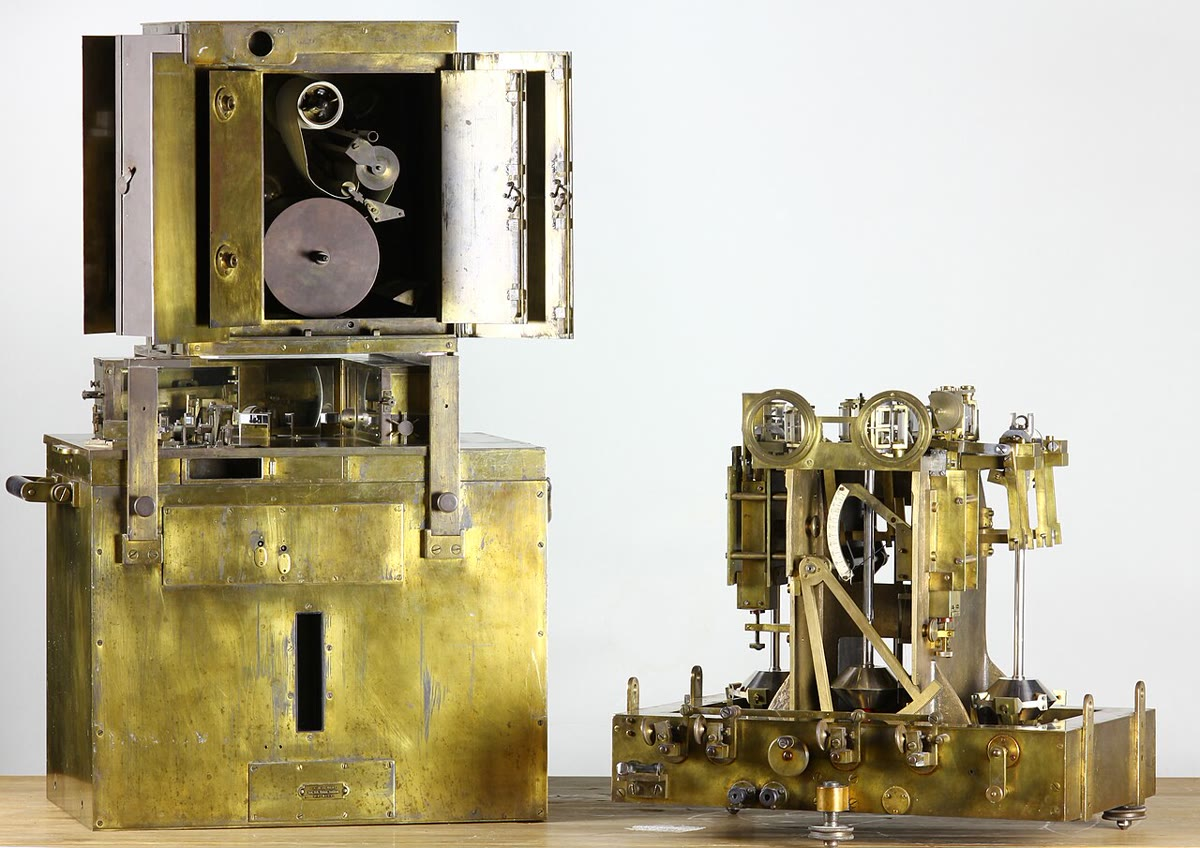
\includegraphics[width=\linewidth]{images/book3/b1-vening-meinesz.jpg}

{\scriptsize 韦宁·梅内斯摆仪（右）及其箱体，
所配记录单元（Broodt，CC BY-SA 4.0）。}
\end{minipage}
\end{history}

\section{大地水准面}

静止的海面是重力势为常数的面：若不是，
水就会沿其流动。它是高程的天然基准，
也是旧时铅垂线所垂直的那个面。

\begin{definition}[大地水准面；大地水准面高]\label{def:b1:isostasy-gravity:geoid}
\emph{大地水准面}\index{大地水准面}是地球重力场的等势面，
此处的重力指引力与自转离心效应之和，
它与开阔大洋上静止的平均海面重合，
并向大陆之下延拓。\emph{大地水准面高}\index{大地水准面高} $N$ 是某点处大地水准面
在参考椭球面之上的高度，
在大地水准面位于椭球面之下处取负值。
\end{definition}

地图上标注的\omterm{def:b1:spherical-astronomy:horizontal}{海拔}高度是相对\omterm{def:b1:isostasy-gravity:geoid}{大地水准面}的高度；卫星定位给出的
高度则是相对椭球面的高度，两者相差
$N$。\omterm{def:b1:isostasy-gravity:geoid}{大地水准面}相对椭球面的偏离，在冰岛附近为 \qty{+85}{m}，
在印度南部近海为 \qty{-106}{m}，总体不超过 \qty{200}{m}，而
固体表面的起伏约 \qty{20}{km}：\omterm{def:b1:isostasy-gravity:geoid}{大地水准面}
是一个比地面光滑得多的面。
% ledger: nasa:geoid-range, earth:topo

\begin{proposition}[大地水准面高与势异常]\label{prop:b1:isostasy-gravity:bruns}
设 $\Phi$ 为地球的重力势，$\Phi_n$ 为正常势，
即模型地球的势，该模型地球的表面（参考椭球面）与\omterm{def:b1:isostasy-gravity:geoid}{大地水准面}具有相同的
势 $\Phi_0$，两者都按物理学的符号取值（势向上增大，
且 $g = -\nabla\Phi$）。设 $T = \Phi - \Phi_n$ 为\omterm{def:b1:isostasy-gravity:geoid}{大地水准面}上的
势异常，则到一阶近似有
\[
  N = -\frac{T}{\gamma} .
\]
大地测量学者取势的符号与此相反，他们把同一结果写作
$N = T/\gamma$，即布伦斯公式。
\end{proposition}

\begin{proof}
设 $Q$ 为椭球面上一点，$P$ 为\omterm{def:b1:isostasy-gravity:geoid}{大地水准面}上的点，
位于过 $Q$ 的法线上、高度为 $N$ 处。正常势向上增大，
变化率为 $\gamma$，故 $\Phi_n(P) \approx \Phi_n(Q) + \gamma N = \Phi_0 +
\gamma N$。由于 $P$ 在\omterm{def:b1:isostasy-gravity:geoid}{大地水准面}上，$\Phi(P) = \Phi_0$，即
$\Phi_n(P) + T = \Phi_0$。由此 $\Phi_0 + \gamma N + T = \Phi_0$，并得 $N =
-T/\gamma$。
\end{proof}

某点之下的质量过剩使该处的势更负，因此
$T < 0$，$N > 0$：\omterm{def:b1:isostasy-gravity:geoid}{大地水准面}在质量过剩之上隆起，在
质量亏损处下沉。冰岛附近的 \qty{85}{m} 隆起对应的势
异常为 $-\qty{85}{m}\times\qty{9.8}{m.s^{-2}} \approx \qty{-830}{J.kg^{-1}}$。
由于势按 $1/r$ 衰减，而引力按 $1/r^2$ 衰减，
\omterm{def:b1:isostasy-gravity:geoid}{大地水准面}主要由大而深的质量决定，\omterm{def:b1:isostasy-gravity:anomalies}{重力异常}则
主要由浅层质量决定。补偿的山脉仅使\omterm{def:b1:isostasy-gravity:geoid}{大地水准面}稍有抬升，
因为其质量过剩与山根的亏损几乎相互抵消；一个
未经补偿的载荷使其抬升得多。

\begin{omfigure}
\begin{tikzpicture}[x=1.15cm, y=1.3cm, font=\scriptsize, >={Stealth[length=4pt]}]
% schematic, not to scale
\fill[omSea!35] (0,0.05) .. controls (1.5,0.25) and (2.5,0.35) .. (3.6,0.45) -- (3.6,-1.2) -- (0,-1.2) -- cycle;
\fill[omLithGranite!40] (3.6,0.45) .. controls (4.5,1.4) and (5.4,1.9) .. (6.4,1.7) .. controls (7.4,1.5) and (8.2,1.2) .. (9,1.0) -- (9,-1.2) -- (3.6,-1.2) -- cycle;
\fill[omLithGabbro!35] (0,-0.7) .. controls (1.2,-0.9) and (2.4,-0.6) .. (3.6,-0.2) -- (3.6,-1.2) -- (0,-1.2) -- cycle;
\draw[thick, blue!70!black] (0,0.05) .. controls (1.5,0.25) and (2.5,0.35) .. (3.6,0.45) .. controls (5,0.75) and (7,0.75) .. (9,0.55);
\draw[thick, black, densely dashed] (0,-0.25) .. controls (3,0.05) and (6,0.15) .. (9,0.1);
\draw (3.6,0.45) .. controls (4.5,1.4) and (5.4,1.9) .. (6.4,1.7) .. controls (7.4,1.5) and (8.2,1.2) .. (9,1.0);
\node[anchor=west, blue!70!black] at (9.05,0.6) {大地水准面};
\node[anchor=west] at (9.05,0.1) {椭球面};
\node[anchor=west] at (9.05,1.0) {地面};
\node at (1.4,-0.3) {海洋};
\node at (1.6,-1.0) {海底};
% heights (curve ordinates computed from the Bezier segments)
\draw[<->] (6.6,0.107) -- (6.6,0.688); \node[anchor=east] at (6.57,0.40) {$N$};
\draw[<->] (7.2,0.674) -- (7.2,1.512); \node[anchor=west] at (7.23,1.09) {$H$};
\draw[<->] (8.2,0.110) -- (8.2,1.224); \node[anchor=east] at (8.17,0.95) {$h_e$};
% the vertical (perpendicular to the geoid) and the ellipsoid normal at x = 2.4 (angle exaggerated)
\draw[->, thick, blue!70!black] (2.4,0.335) -- (2.0,1.3);
\draw[->, thick, black] (2.4,0.335) -- (2.33,1.3);
\node[anchor=south east, blue!70!black] at (2.05,1.3) {竖直方向（铅垂线）};
\node[anchor=south west] at (2.3,1.3) {椭球法线};
\end{tikzpicture}

\par\smallskip{\small \omterm{def:b1:isostasy-gravity:geoid}{大地水准面}（蓝色）、参考椭球面（虚线）与
地面（示意图；偏差被大大夸大）。在海洋上，\omterm{def:b1:isostasy-gravity:geoid}{大地水准面}
即静止的海面；在陆地之下，它延拓为等势面。
地图上的高度 $H$ 从\omterm{def:b1:isostasy-gravity:geoid}{大地水准面}量起，卫星定位给出的高度 $h_e$
则从椭球面量起，且 $h_e = H + N$。铅垂线
垂直于\omterm{def:b1:isostasy-gravity:geoid}{大地水准面}，而非椭球面：二者之间的夹角
（此处已夸大）即是
困扰印度测量人员的垂线偏差。}
\label{fig:b1:isostasy-gravity:geoid}
\end{omfigure}

垂线偏差很小：困扰
印度测量人员的全部偏差约为五角秒。在海洋上，\omterm{def:b1:isostasy-gravity:geoid}{大地水准面}是可以观测到的。
自 1978 年起，卫星上的雷达高度计便对
从海面反射的微波脉冲计时，以测定海面高度。潮汐、波浪和
洋流被平均掉之后，海面在海山与洋脊之上较高，
在海沟与深海平原之上较低，这些起伏（\cref{exo:b1:isostasy-gravity:11}
估算其一）可描绘出从未有船只测深的深海海底地形。
卫星 GOCE 于 2009 至 2013 年间在约 \qty{260}{km} 高度飞行，
并从轨道上测量重力场，目标是将\omterm{def:b1:isostasy-gravity:geoid}{大地水准面}精度达到 1 至
\qty{2}{cm}，\omterm{def:b1:isostasy-gravity:anomalies}{重力异常}精度约为 \qty{1}{\milli\gal}，并具有
优于 \qty{100}{km} 的分辨率。
% ledger: pratt:himalaya, jpl:seasat, esa:goce

\subsection*{运动中的地壳均衡}

\omterm{def:b1:isostasy-gravity:isostasy}{地壳均衡}通过流动达成，而流动需要时间。在上一次冰期的顶峰
时，约 \num{20000} 年前，一层厚约 \qty{3}{km} 的冰盖
覆盖了斯堪的纳维亚半岛。
冰的密度约为水的十分之九，因此取\omterm{def:b1:layered-earth:layers}{地幔}密度为
\qty{3300}{kg.m^{-3}}，则此类冰盖下的完全均衡下沉量为
$\qty{3000}{m}\times900/3300 \approx \qty{820}{m}$。冰盖已消失，而
陆地仍在抬升：卫星定位测得
瑞典北部（波的尼亚湾以西）的抬升速率高达约 \qty{10}{mm.\text{年}^{-1}}，
至今。冰盖下陷的
松弛速率测定了其下方\omterm{def:b1:layered-earth:layers}{地幔}的黏度，
此为第 5 册的主题；\cref{exo:b1:isostasy-gravity:12} 说明了方法。
% ledger: kierulf:fennoscandia, usgs:ice-density

\section{练习}

\begin{exercise}[$\star$]\label{exo:b1:isostasy-gravity:1}
(a) 将\omterm{def:b1:isostasy-gravity:anomalies}{布格异常} \qty{-150}{\milli\gal} 换算为 \unit{m.s^{-2}}，
并将其表示为 $g = \qty{9.81}{m.s^{-2}}$ 的分数。(b) 对
\qty{1}{\milli\gal}（GOCE \omterm{def:b1:isostasy-gravity:anomalies}{重力异常}所追求的精度）及
\qty{1}{\micro\gal} 做同样的计算。
% ledger: esa:goce, nist:gal
\end{exercise}

\begin{exercise}[$\star$]\label{exo:b1:isostasy-gravity:2}
(a) 计算赤道、\ang{45} 处及两极的\omterm{def:b1:isostasy-gravity:normal-gravity}{正常重力}，
所用公式为本章公式。(b) 以毫伽为单位给出赤道与两极之间的差值。
(c) 赤道处的离心加速度为
\qty{3392}{\milli\gal}，问自转直接解释了
差值的多大比例？
% ledger: moritz:grs80
\end{exercise}

\begin{exercise}[$\star$]\label{exo:b1:isostasy-gravity:3}
某高原高出海平面 \qty{3}{km}，\omterm{def:b1:layered-earth:layers}{地壳}密度为
\qty{2800}{kg.m^{-3}}，\omterm{def:b1:layered-earth:layers}{地幔}密度为 \qty{3300}{kg.m^{-3}}，求其艾里根
及\omterm{def:b1:layered-earth:layers}{地壳}增厚量。
\end{exercise}

\begin{exercise}[$\star$]\label{exo:b1:isostasy-gravity:4}
(a) 重力仪须升高多少，读数才会减小
\qty{1}{\milli\gal}？取 \qty{0.3086}{\milli\gal.m^{-1}}。(b) 某测量拟使
异常精度达到 \qty{0.01}{\milli\gal}，则测站高度
须精确到多少？
\end{exercise}

\begin{exercise}[$\star\star$]\label{exo:b1:isostasy-gravity:5}
在普拉特模型中，取 $D = \qty{100}{km}$ 及 $\rho_0 = \qty{2700}{kg.m^{-3}}$，
(a) 求高度分别为 1、3 及 \qty{5}{km} 的柱体密度；
(b) 求位于 \qty{4}{km} 厚海水之下的柱体密度，海水密度为
\qty{1030}{kg.m^{-3}}。(c) 为何普拉特模型更适用于洋底，
而非大陆？
\end{exercise}

\begin{exercise}[$\star\star$]\label{exo:b1:isostasy-gravity:6}
两测站位于\omterm{def:b1:spherical-astronomy:geographic}{纬度} \ang{48}，该处\omterm{def:b1:isostasy-gravity:normal-gravity}{正常重力}为
\qty{9.808911}{m.s^{-2}}。测站 1 位于\omterm{def:b1:spherical-astronomy:horizontal}{海拔} \qty{350}{m}，读数为
\qty{9.807751}{m.s^{-2}}；测站 2 位于 \qty{1850}{m}，读数为
\qty{9.803552}{m.s^{-2}}。(a) 求两站的\omterm{def:b1:isostasy-gravity:anomalies}{自由空气异常}与\omterm{def:b1:isostasy-gravity:anomalies}{布格异常}，
取标准布格密度。(b) 测站 2 的异常对其周围的山体
有何启示？
\end{exercise}

\begin{exercise}[$\star\star$]\label{exo:b1:isostasy-gravity:7}
(a) 仿照\cref{prop:b1:isostasy-gravity:slab}的证明，说明
半径为 $a$、厚度为 $h$、密度为 $\rho$ 的水平圆盘，
对其轴线上、上方距离 $z \gg h$ 处的一点的引力为 $2\pi G\rho h\,\bigl(1 -
z/\sqrt{z^2 + a^2}\bigr)$。(b) 半径取何值时，可使 \qty{90}{\percent} 的板片
值出现于 $z = \qty{1}{km}$ 处？(c) 这对\omterm{def:b1:isostasy-gravity:anomalies}{布格校正}有关的地形范围说明了
什么？
\end{exercise}

\begin{exercise}[$\star\star$]\label{exo:b1:isostasy-gravity:8}
在艾里模型中，\omterm{def:b1:layered-earth:layers}{地壳}密度为 \qty{2800}{kg.m^{-3}}，海平面处厚 \qty{35}{km}，
位于密度为 \qty{3300}{kg.m^{-3}} 的\omterm{def:b1:layered-earth:layers}{地幔}之上。(a) 求反根及
在厚 \qty{4}{km}、密度为 \qty{1030}{kg.m^{-3}} 的海水之下的\omterm{def:b1:layered-earth:layers}{地壳}厚度。
(b) 实际洋壳厚约 \qty{5}{km}。这一
差异说明了什么？% ledger: usgs:crust-thickness
\end{exercise}

\begin{exercise}[$\star\star$]\label{exo:b1:isostasy-gravity:9}
在开篇的叙述中，卡利亚纳与卡利安普尔之间\omterm{def:b1:spherical-astronomy:geographic}{纬度}差的偏差
为 \qty{5.236}{''}，而按普拉特模型计算的喜马拉雅山吸引力
本应产生 \qty{15.885}{''}。(a) 将
两角均换算为弧度。(b) 水平加速度 $a_h$ 使铅垂线偏转
角度 $a_h/g$。两测站间水平引力之差
各角对应多少，以毫伽计，取
$g = \qty{9.79}{m.s^{-2}}$？(c) 补偿作用抵消了
可见山体引力的多大比例？
% ledger: pratt:himalaya
\end{exercise}

\begin{exercise}[$\star\star\star$]\label{exo:b1:isostasy-gravity:10}
盐丘被模拟为半径为 \qty{2}{km} 的球体，球心位于
\qty{4}{km} 深处，其密度比周围岩石低
\qty{200}{kg.m^{-3}}。(a) 证明：异常质量为 $M$ 的球体埋藏于深度 $z$ 处，
在水平距离 $x$ 处给出异常 $GMz/(x^2 + z^2)^{3/2}$。
(b) 求其球心正上方的异常。(c) 在何距离处，
异常降至峰值的一半？(d) 如何由
实测剖面读出球体的深度？
\end{exercise}

\begin{exercise}[$\star\star\star$]\label{exo:b1:isostasy-gravity:11}
海山是一个高 \qty{3}{km}、底面半径为 \qty{15}{km} 的锥体，
立于深 \qty{5}{km} 的海底之上。其岩石密度为
\qty{2800}{kg.m^{-3}}，海水密度为 \qty{1030}{kg.m^{-3}}。(a) 求其
相对于所排开海水的超额质量。(b) 将其视为一质点，位于质心处，
该质心位于底面以上高度的四分之一处，并利用
\cref{prop:b1:isostasy-gravity:bruns}，取 $\gamma = \qty{9.81}{m.s^{-2}}$，估算
其上方海面隆起的高度。(c) 该质点模型
高估还是低估了隆起？(d) 若海山由根完全补偿，
隆起将如何变化？
\end{exercise}

\begin{exercise}[$\star\star\star$]\label{exo:b1:isostasy-gravity:12}
建立冰消后斯堪的纳维亚半岛回弹的模型：设冰层
于 \num{10000} 年前突然消失，留下 \qty{818}{m} 的下沉量，此后该下沉量
按 $w(t) = w_0\,e^{-t/\tau}$ 减小。(a) 证明抬升速率为
$w/\tau$。(b) 取 $\tau = \num{4000}$ 年，求剩余下沉量
及今日的抬升速率，并将该速率与实测的
\qty{10}{mm.\text{年}^{-1}} 相比较。(c) 证明 $\tau = \num{3100}$ 年与
$\tau = \num{68000}$ 年均给出今日约 \qty{10}{mm.\text{年}^{-1}} 的速率。
各自对应的剩余下沉量为多少，重力测量如何判定
两者之中何者成立？(d) $\tau$ 所度量的是\omterm{def:b1:layered-earth:layers}{地幔}的何种性质？
% ledger: kierulf:fennoscandia
\end{exercise}

\section{问题：山脉之根}

\begin{problem}[{周末问题——高原之根，艾里与普拉特之争，
其上的重力，以及侵蚀的影响}]
\label{pb:b1:isostasy-gravity:1}
% values: calc/ch11.py (invented plateau; normal gravity formula of the chapter)
% ledger: moritz:grs80, usgs73:reduction
一块宽达数百千米的高原，比海平面上的低地高出 \qty{4}{km}，
该低地\omterm{def:b1:layered-earth:layers}{地壳}厚 \qty{35}{km}。取
\omterm{def:b1:layered-earth:layers}{地壳}密度 $\rho_c = \qty{2700}{kg.m^{-3}}$，\omterm{def:b1:layered-earth:layers}{地幔}密度 $\rho_m = \qty{3300}{kg.m^{-3}}$，
$g = \qty{9.81}{m.s^{-2}}$，且
$2\pi G = \qty{0.0419}{\milli\gal}$ 每米每 \qty{1000}{kg.m^{-3}}。

\medskip
\noindent\textbf{第一部分——艾里高原。}
\begin{enumerate}
  \item 计算该高原的艾里根。
  \item 推出其\omterm{def:b1:layered-earth:layers}{地壳}厚度，以及其\omterm{def:b1:layered-earth:discontinuity}{莫霍面}
        在海平面以下的深度。
  \item 取\omterm{def:b1:isostasy-gravity:isostasy}{补偿深度}为海平面以下 \qty{60}{km}，
        计算高原柱体与低地柱体在其上方
        每平方米的质量。
  \item 计算 \qty{60}{km} 深处的压强。
  \item 为何根部是高度的 4.5 倍？若
        \omterm{def:b1:layered-earth:layers}{地壳}密度为 \qty{2900}{kg.m^{-3}}，则比值为多少？
  \item 若艾里模型成立，横跨高原边缘的地震折射
        测量会显示什么？
\end{enumerate}

\noindent\textbf{第二部分——普拉特高原。}
现设\omterm{def:b1:isostasy-gravity:isostasy}{补偿深度}为海平面以下 $D = \qty{100}{km}$，
且低地柱体密度均匀，为 \qty{2700}{kg.m^{-3}}。
\begin{enumerate}[resume]
  \item 计算高原柱体的密度。
  \item 验证两柱体在
        $D$ 以上每平方米的质量相同。
  \item 高原柱体须轻多少，以百分数表示？
  \item 若该密度差仅由热效应引起，
        热膨胀系数为 \qty{3e-5}{K^{-1}}，则高原柱体平均
        须升温多少？这是否合理？
  \item 在普拉特模型中，高原之下的\omterm{def:b1:layered-earth:discontinuity}{莫霍面}位于何处？
  \item 折射测量发现高原之下的\omterm{def:b1:layered-earth:discontinuity}{莫霍面}位于 \qty{52}{km} 处，
        哪一种模型与之相符？
\end{enumerate}

\noindent\textbf{第三部分——中心处的重力。}
\begin{enumerate}[resume]
  \item 计算高原上某测站的\omterm{def:b1:isostasy-gravity:anomalies}{布格校正}。
  \item 若高原未被补偿，预测
        高原中心处的\omterm{def:b1:isostasy-gravity:anomalies}{自由空气异常}与\omterm{def:b1:isostasy-gravity:anomalies}{布格异常}。
  \item 对艾里高原作同样预测，并以
        根部缺失的质量核对\omterm{def:b1:isostasy-gravity:anomalies}{布格异常}。
  \item 高原中心处一测站位于\omterm{def:b1:spherical-astronomy:geographic}{纬度} \ang{30}，
        \omterm{def:b1:spherical-astronomy:horizontal}{海拔} \qty{4000}{m}，读数为 \qty{9.781085}{m.s^{-2}}。计算
        \omterm{def:b1:spherical-astronomy:geographic}{纬度} \ang{30} 处的\omterm{def:b1:isostasy-gravity:normal-gravity}{正常重力}，再求\omterm{def:b1:isostasy-gravity:anomalies}{自由空气异常}与\omterm{def:b1:isostasy-gravity:anomalies}{布格异常}。
  \item 高原中被补偿的部分占多大比例？
  \item 若高原按普拉特方式补偿，中心处的
        \omterm{def:b1:isostasy-gravity:anomalies}{布格异常}是否会不同？试说明理由。
  \item 绘出穿过高原某一边缘的剖面上
        \omterm{def:b1:isostasy-gravity:anomalies}{自由空气异常}的示意图，并解释其形状。
\end{enumerate}

\noindent\textbf{第四部分——侵蚀。}
河流自高原整个表面移去一层厚 \qty{1}{km} 的岩层，
移去速度足够缓慢，以使\omterm{def:b1:isostasy-gravity:isostasy}{地壳均衡}得以跟上。
\begin{enumerate}[resume]
  \item \omterm{def:b1:layered-earth:layers}{地壳}的新厚度为多少，其新的艾里根为多少？
  \item 高原的新\omterm{def:b1:spherical-astronomy:horizontal}{海拔}为多少？
  \item 如今位于地表的岩石已上升了多少？
  \item 总共须侵蚀掉多少岩石，才能使高原降至
        海平面？这对古老造山带中所见的岩石说明了什么？
  \item 每侵蚀一千米岩石，
        高原表面下降多少？
\end{enumerate}
\end{problem}
